\section{Árvore AVL}
\label{sec:avl}

Esta se trata de uma implementação balanceada de uma BST. Sua primeira menção é datada no ano de 1962, no artigo \textbf{An algorithm for organization of information}, dos autores Georgy Maximovich \textbf{A}delson-\textbf{V}elsky e Evgenii Mikhailovich \textbf{L}andis, cujas iniciais foram eternizadas na nomeação do conceito. Sendo assim, sua intenção minimizar a complexidade da operação de busca, enquanto aumenta um pouco o custo da inserção e remoção, e isso acontece através do conceito de rotações.

E sabendo do conceito de balanceamento apresentado anteriormente, o critério usado para aplicá-lo é o chamado \textbf{Fato de Balanceamento}, que pode ser formalizado da seguinte forma
\begin{align*}
   (\forall t \in \text{AVLTree } \alpha) \quad 
   \left[ \, \text{BF} = \text{height(t.left)} - \text{height(t.right)} \, \right]
\end{align*}

Sendo assim, seja \textbf{n} um nó de uma Árvore AVL, os quatro casos em que o \textbf{Fator de balanceamento} é usado como critério para balancear a árvore são os seguintes:

\begin{itemize}
	\item \textbf{Rotação direita} \\
		Quando temos que \textbf{BF(n) < -1 e height(n.right.left) < height(n.right.right)}, o nó está muito pesado na esquerda, sendo assim é necessária uma que o nó onde o desbalanceamento inicia seja rotacionado à direita. Ou seja, visualmente algo parecido com o exemplo abaixo
	\begin{align*}
		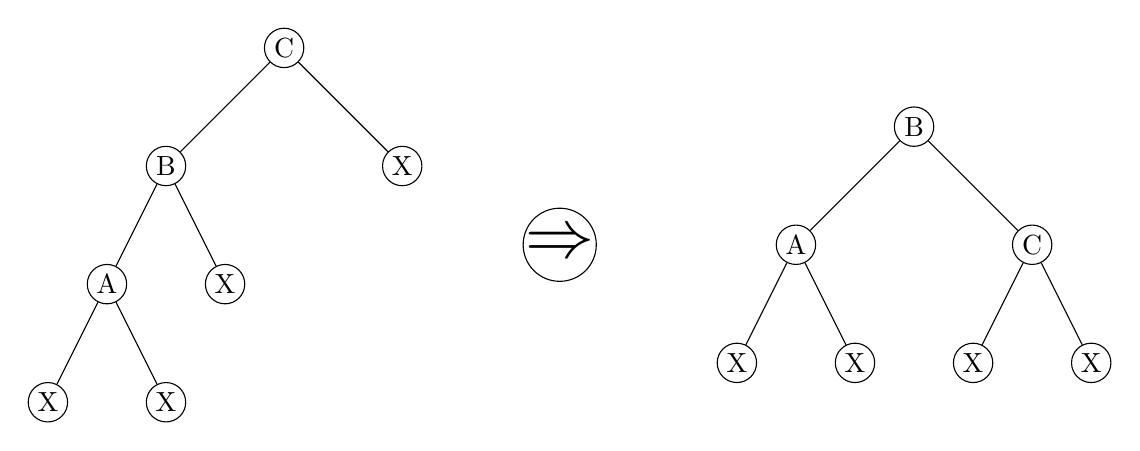
\begin{tikzpicture}[
			every node/.style={circle, draw, minimum size=0.5cm, inner sep=0},
			level 1/.style={sibling distance=3cm},
			level 2/.style={sibling distance=1.5cm},
		]
		\node (tree1) at (0,0) {C}
			child {node {B}
				child {node {A}
					child {node {X}}
					child {node {X}}
				}
				child {node {X}}
			}
			child {node {X}};
			\node[style={}] (arrow) at (3.5,-2.5) {\Huge$\Rightarrow$};
		\node (tree2) at (8,-1) {B}
			child {node {A}
				child {node {X}}
				child {node {X}}
			}
			child {node {C}
				child {node {X}}
				child {node {X}}
			};
		\end{tikzpicture}
	\end{align*}

	\item \textbf{Rotação esquerda} \\
		Quando temos que \textbf{BF(n) > 1 e height(n.left.right) < height(n.left.left)}, há uma sobrecarga na direita do nó, portanto se faz necessária uma rotação à esquerda.
	\begin{align*}
		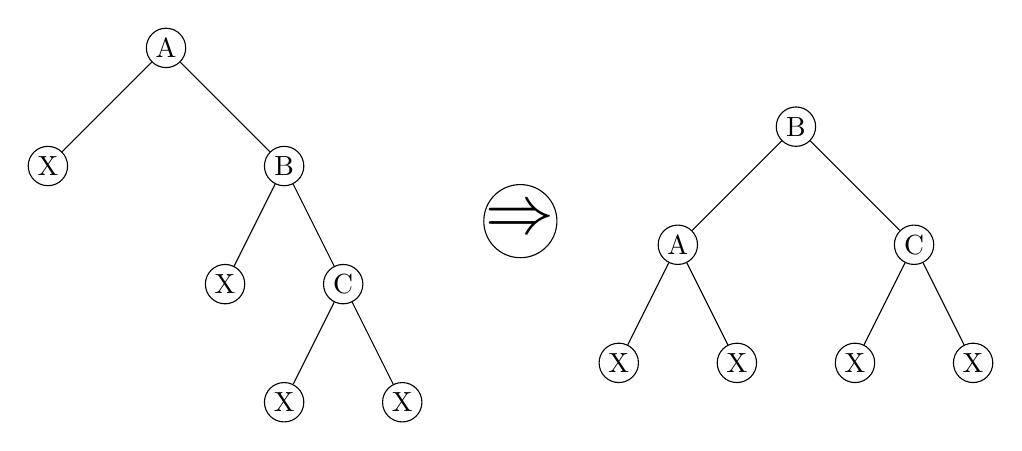
\begin{tikzpicture}[
			every node/.style={circle, draw, minimum size=0.5cm, inner sep=0},
			level 1/.style={sibling distance=3cm},
			level 2/.style={sibling distance=1.5cm},
		]
		\node (tree1) at (0,0) {A}
			child {node {X}
			}
			child {node {B}
				child {node {X}
				}
				child {node {C}
					child {node {X}}
					child {node {X}}
				}
			};
			\node[style={}] (arrow) at (4.5,-2.2) {\Huge$\Rightarrow$};
		\node (tree2) at (8,-1) {B}
			child {node {A}
				child {node {X}}
				child {node {X}}
			}
			child {node {C}
				child {node {X}}
				child {node {X}}
			};
		\end{tikzpicture}
	\end{align*}

	\item \textbf{Rotação direita-esquerda} \\
		Quando temos que \textbf{BF(n) < -1}, o nó à esquerda está muito pesado, entretanto não basta uma uma rotação direita, mas sim uma rotação direita seguida por outra à esquerda.
	\begin{align*}
		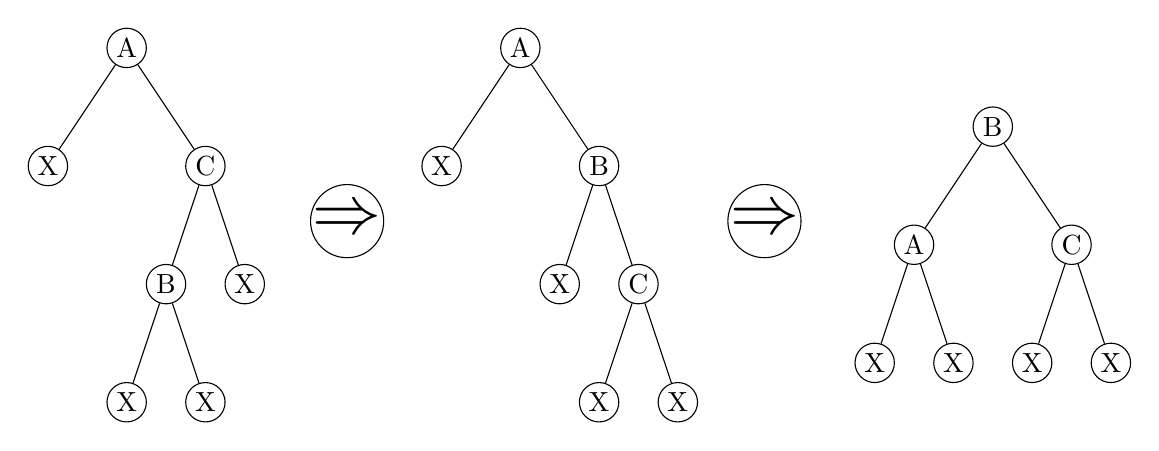
\begin{tikzpicture}[
			every node/.style={circle, draw, minimum size=0.5cm, inner sep=0},
			level 1/.style={sibling distance=2cm},
			level 2/.style={sibling distance=1cm},
		]
		\node (tree1) at (0,0) {A}
			child {node {X}
			}
			child {node {C}
				child {node {B}
					child {node {X}}
					child {node {X}}
				}
				child {node {X}}
			};
			\node[style={}] (arrow) at (2.8,-2.2) {\Huge$\Rightarrow$};
		\node (tree2) at (5,0) {A}
			child {node {X}
			}
			child {node {B}
				child {node {X}
				}
				child {node {C}
					child {node {X}}
					child {node {X}}
				}
			};
			\node[style={}] (arrow) at (8.1,-2.2) {\Huge$\Rightarrow$};
		\node (tree3) at (11,-1) {B}
			child {node {A}
				child {node {X}}
				child {node {X}}
			}
			child {node {C}
				child {node {X}}
				child {node {X}}
			};
		\end{tikzpicture}
	\end{align*}
	\item \textbf{Rotação esquerda-direita} \\
		Quando temos que \textbf{BF(n) > 1}, há uma sobrecarga na direita do nó, entretanto uma rotação esquerda não é suficiente, mas sim uma rotação esquerda seguida por outra à direita.
	\begin{align*}
		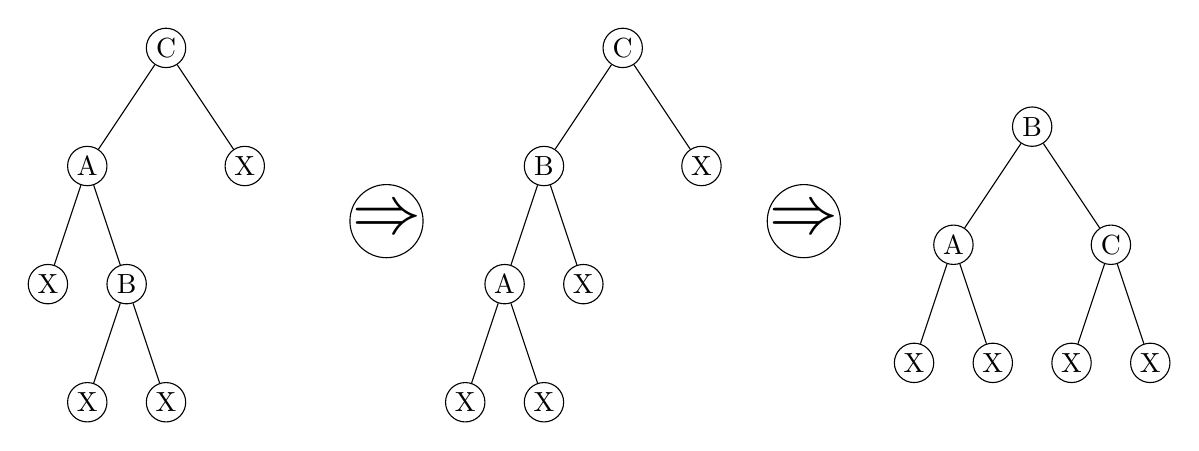
\begin{tikzpicture}[
			every node/.style={circle, draw, minimum size=0.5cm, inner sep=0},
			level 1/.style={sibling distance=2cm},
			level 2/.style={sibling distance=1cm},
		]
		\node (tree1) at (0,0) {C}
			child {node {A}
				child {node {X}
				}
				child {node {B}
					child {node {X}}
					child {node {X}}
				}
			}
			child {node {X}
			};
			\node[style={}] (arrow) at (2.8,-2.2) {\Huge$\Rightarrow$};
		\node (tree2) at (5.8,0) {C}
			child {node {B}
				child {node {A}
					child {node {X}}
					child {node {X}}
				}
				child {node {X}
				}
			}
			child {node {X}
			};
			\node[style={}] (arrow) at (8.1,-2.2) {\Huge$\Rightarrow$};
		\node (tree3) at (11,-1) {B}
			child {node {A}
				child {node {X}}
				child {node {X}}
			}
			child {node {C}
				child {node {X}}
				child {node {X}}
			};
		\end{tikzpicture}
	\end{align*}
\end{itemize}

\subsection{Implementação}

No que diz respeito à implementação, esta foi feita utilizando Haskell, uma linguagem de programação funcional. A estrutura de dado foi implementada da conforme o código abaixo.

\begin{lstlisting}[language=haskell]
data AVLTree a
  = Node
      { key :: a
      , left :: AVLTree a
      , right :: AVLTree a
      }
  | Nil
\end{lstlisting}

Sendo assim, é possível criar instâncias de \texttt{AVLTree a}, onde \texttt{a} é um tipo genérico. Podendo ser através do construtor \texttt{Nil} que representa uma folha vazia, indicando o fim daquele determinado galho. Bem como também pode ser usando o \texttt{Node} que se trata de um nó, que deve receber 3 argumentos: O valor de tipo \texttt{a} que ele vai armazenar e suas sub-árvores esquerda e direita.

A seguir será elucidado como foram implementadas as funções de Inserção, Remoção e Busca.

\subsection{Busca}
Esta se trata da operação que o funcionamento da Árvore AVL acaba privilegiando, seu comportamento é identico à de uma implementação básica de uma BST. Entretanto o balanceamento é um fator importantíssimo para que a função opere com o máximo desempenho, apesar de ser idêntica à uma BST padrão. E isso acontece pois \textbf{apenas} as operações de inserção e remoção podem balancear a árvore, sendo assim, esta já está em seu melhor cenário de distribuição de elementos quando uma busca é iniciada.
A operação foi implementada conforme a seguir.

\begin{lstlisting}[language=haskell]
search :: (Ord a) => AVLTree a -> a -> Maybe [Direction]
search Nil _ = Nothing
search (Node k l r) v
    | v == k = Just []
    | v <= k = fmap (L :) (search l v)
    | otherwise = fmap (R :) (search r v)
\end{lstlisting}

Esta implementação tem algumas particularidades, a primeira delas sendo que ao invés de retornar apenas um booleano correspondente à existência de determinado elemento naquela instância de de \texttt{AVLTree a}, esta retorna a lista de direções que leva até ele.

Também note que ela utiliza o \texttt{Maybe a}, que é um tipo genérico que tem dois construtores: O \texttt{Nothing} e o \texttt{Just x}. Em que o \texttt{Nothing} é uma forma segura de dizer que não há correspondente ao que se procura, semelhante à uma exceção. Já o \texttt{Just x} é uma mera forma de encapsular um retorno bem sucedido da operação.

Por fim, também é usado o conceito de \texttt{Typeclass} através do \texttt{Ord a}, sendo esse um conceito dentro da Haskell para tipos que atendem a determinadas especificações. Em especial a \texttt{Ord a} se trata de uma "família" de tipos cujos valores são ordenáveis, o que torna possível a operação >, que orienta as direções da busca. Em síntese, já que a Árvore AVL é extremamente dependente de comparações ordenáveis, não faz sentido que \texttt{a} seja um tipo como Bool, por exemplo.
\subsection{Inserção}

Se tratando a Árvore AVL, a inserção está longe de ser uma das suas operações mais eficientes, e isso acontece pois ela é responsável por balancear a árvore pós-inserção. Ou seja, podemos dividir a inserção em duas partes: Inserir de forma bruta e balancear a árvore uma vez feita a inserção. Sendo assim, o primeiro passo é muito bem retratado pela função \texttt{insert'} abaixo.

\begin{lstlisting}[language=haskell]
insert' :: (Ord a) => a -> AVLTree a -> AVLTree a
insert' v Nil = Node v Nil Nil
insert' v (Node v' l r)
    | v' <= v = Node v' l (insert' v r)
    | otherwise = Node v' (insert' v l) r
\end{lstlisting}

Em síntese, ela se comporta praticamente igual à busca, com a ressalva de que ela só para quando chega em uma folha vazia, e faz a sobrescrita do \texttt{Nil} para que este vire um \texttt{Node (valor Nil Nil)}.

Entretanto, após isso é necessário se certificar que se um balanceamento se faz necessário. Nesse caso podemos dividir o ato de balancear em duas partes: Verificar qual o nó que causa o desbalanceamento(caso ele exista) e rotacioná-lo. Essas funções são respectivamente atribuídas às funções \texttt{findUnbalancedNode} e \texttt{rotateAt}

\begin{lstlisting}[language=haskell]
insert :: (Ord a) => a -> AVLTree a -> AVLTree a
insert v t =
    let treeAfterInsertion = insert' v t
     in rotateAt treeAfterInsertion (findUnbalancedNode treeAfterInsertion)

findUnbalancedNode :: (Ord a) => AVLTree a -> Maybe [Direction]
findUnbalancedNode Nil = Nothing
findUnbalancedNode t@(Node v l r)
    | balanced t = Nothing
    | not (balanced t) && balanced l && balanced r = Just []
    | balanced l = fmap (R :) (findUnbalancedNode r)
    | otherwise = fmap (L :) (findUnbalancedNode l)

rotateAt :: (Ord a) => AVLTree a -> Maybe [Direction] -> AVLTree a
rotateAt t Nothing = t
rotateAt (Node v l r) (Just (d : ds)) = case d of
    R -> Node v l (rotateAt r (Just ds))
    L -> Node v (rotateAt l (Just ds)) r
rotateAt t (Just []) = rotateNode t
\end{lstlisting}

Ademais, também são usadas as funções auxiliares abaixo. Sendo a \texttt{rotateNode} responsável por fazer a rotação cabível, uma vez que há a garantia que ela está no nó que causa do desbalanceamento. Bem como as demais funções são as rotações simples e duplas.

\begin{lstlisting}[language=haskell]
rotateNode :: (Ord a) => AVLTree a -> AVLTree a
rotateNode Nil = Nil
rotateNode t@(Node _ l r)
    | balanceFactor < -1 && height (left r) < height (right r)
        =
        trace "Rotation R" rotateR t
    | balanceFactor > 1 && height (right l) < height (left l)
        =
        trace "Rotation L" rotateL t
    | balanceFactor < -1 && height (left r) > height (right r)
        =
        trace "Rotation RL" rotateRL t
    | balanceFactor > 1 && height (right l) > height (left l)
        =
        trace "Rotation LR" rotateLR t
  where
    balanceFactor = height l - height r

rotateR :: (Ord a) => AVLTree a -> AVLTree a
rotateR (Node e l (Node er lr rr)) = Node er (Node e l lr) rr

rotateL :: (Ord a) => AVLTree a -> AVLTree a
rotateL (Node e (Node el ll rl) r) = Node el ll (Node e rl r)

rotateLR :: (Ord a) => AVLTree a -> AVLTree a
rotateLR (Node e (Node el ll (Node elr lrl lrr)) r) = Node elr (Node el ll lrl) (Node e lrr r)

rotateRL :: (Ord a) => AVLTree a -> AVLTree a
rotateRL (Node e l (Node er (Node erl rll rlr) rr)) = Node erl (Node e l rll) (Node er rlr rr)
\end{lstlisting}

\subsection{Remoção}

Por fim, a remoção talvez se trate da complexa entre as operações. Isso pois seu balanceamento envolve mais elementos do que meramente rotacionar a árvore. Entretanto, podemos separá-la nos três seguintes casos

\begin{itemize}
	\item \textbf{Remoção de um nó sem filhos} \\
		Esse caso é trivial, basta substituir um \texttt{Node} que contenha o valor a ser removido por um \texttt{Nil}. Suponha que o \textbf{C} é o elemento a ser removido.

		\begin{align*}
			\begin{tikzpicture}[
				every node/.style={circle, draw, minimum size=0.5cm, inner sep=0},
				level 1/.style={sibling distance=3cm},
				level 2/.style={sibling distance=1.5cm},
			]
			\node (tree1) at (0,0) {A}
				child {node {X}
				}
				child {node {B}
					child {node {X}
					}
					child {node {C}
						child {node {X}}
						child {node {X}}
					}
				};
				\node[style={}] (arrow) at (4.5,-2.2) {\Huge$\Rightarrow$};
			\node (tree2) at (8,-1) {A}
				child {node {X}
				}
				child {node {B}
					child {node {X}
					}
					child {node {X}
					}
				};
			\end{tikzpicture}
		\end{align*}
	\item \textbf{Remoção de um nó com um filho} \\
		Nesse caso, independente se o nó tem uma sub-árvore esquerda ou direita, é feita uma ligação direta entre seu filho e seu avô. Suponha que \textbf{B} é o elemento a ser removido.
		\begin{align*}
			\begin{tikzpicture}[
				every node/.style={circle, draw, minimum size=0.5cm, inner sep=0},
				level 1/.style={sibling distance=3cm},
				level 2/.style={sibling distance=1.5cm},
			]
			\node (tree1) at (0,0) {A}
				child {node {X}
				}
				child {node {B}
					child {node {X}
					}
					child {node {C}
						child {node {X}}
						child {node {X}}
					}
				};
				\node[style={}] (arrow) at (4.5,-2.2) {\Huge$\Rightarrow$};
			\node (tree2) at (8,-1) {A}
				child {node {X}
				}
				child {node {C}
					child {node {X}
					}
					child {node {X}
					}
				};
			\end{tikzpicture}
		\end{align*}
	\item \textbf{Remoção da um nó com dois filhos} \\
		Nesse caso precisaremos substituir o valor do nó pelo valor de uma folha, podendo ser tanto o menor valor da sub-árvore direita ou o maior da sub-árvore esquerda, geralmente usa-se o primeiro método. Suponha que o \textbf{D} deve ser removido.
		\begin{align*}
			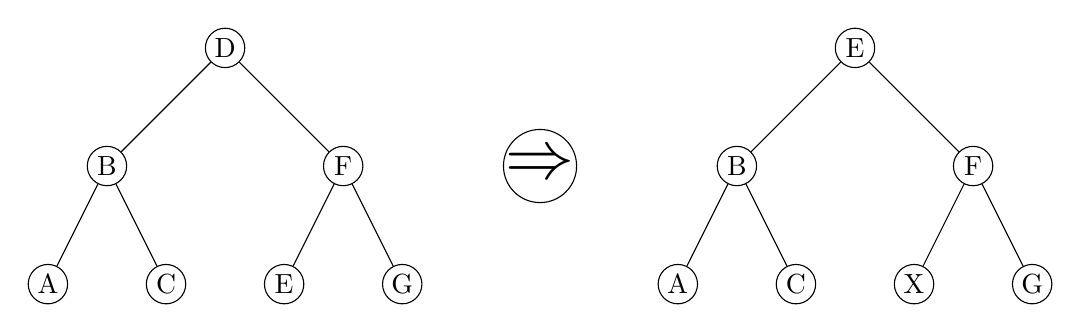
\begin{tikzpicture}[
				every node/.style={circle, draw, minimum size=0.5cm, inner sep=0},
				level 1/.style={sibling distance=3cm},
				level 2/.style={sibling distance=1.5cm},
			]
			\node (tree1) at (0,0) {D}
				child {node {B}
					child {node {A}}
					child {node {C}}
				}
				child {node {F}
					child {node {E}
					}
					child {node {G}
					}
				};
				\node[style={}] (arrow) at (4.0,-1.5) {\Huge$\Rightarrow$};
			\node (tree2) at (8,0) {E}
				child {node {B}
					child {node {A}}
					child {node {C}}
				}
				child {node {F}
					child {node {X}
					}
					child {node {G}
					}
				};
			\end{tikzpicture}
		\end{align*}
\end{itemize}

Apresentados os casos mais triviais, vale ressaltar que as implementações reais também envolvem o balanceamento pós-remoção, conforme feito no código abaixo. Nele fora usadas, além das funções já apresentadas anteriormente, as funções \texttt{remove}, \texttt{remove'} e \texttt{removeMin}. Que respectivamente fazem o balanceamento pós-remoção, a remoção de fato e a busca e remoção do menor elemento da sub-árvore direita.

\begin{lstlisting}[language=haskell]
remove :: (Ord a) => a -> AVLTree a -> AVLTree a
remove v t =
    let treeAfterRemotion = remove' v t
     in rotateAt treeAfterRemotion (findUnbalancedNode treeAfterRemotion)

remove' :: (Ord a) => a -> AVLTree a -> AVLTree a
remove' _ Nil = Nil
remove' n t@(Node v Nil Nil)
    | n == v = Nil
    | otherwise = trace "Element does not exist" t
remove' n (Node v l Nil)
    | n == v = l
    | n < v = Node v (remove' n l) Nil
    | otherwise = trace "Element does not exist" (Node v l Nil)
remove' n (Node v Nil r)
    | n == v = r
    | n > v = Node v Nil (remove' n r)
    | otherwise = trace "Element does not exist" (Node v Nil r)
remove' n (Node v l r)
    | n < v = Node v (remove' n l) r
    | n > v = Node v l (remove' n r)
    | n == v =
        let (successor, newRight) = removeMin r
         in Node successor l newRight

removeMin :: (Ord a) => AVLTree a -> (a, AVLTree a)
removeMin (Node v Nil r) = (v, r)
removeMin (Node v l r) =
    let (minValue, newLeft) = removeMin l
     in (minValue, Node v newLeft r)
\end{lstlisting}

Em súmula, observamos que a Árvore AVL é uma implementação que privilegia a operação de busca pois terceiriza o balanceamento para as operações de inserção e remoção. Isso implica em um maior custo computacional para executar as últimas duas, entretanto nada tão significativo, pois, no fim, ambas as três tem complexidade \textbf{O(log n)}.
